\section{问题分析}

四个问题表面上分别问温度、含水率、时长和收缩，实质上共用同一副骨架：药材内部的热量与水分各自满足一条守恒律，表面通过对流与烘房空气交换，轴线因对称而无净通量。真正逐问变化的只有三样东西，即物性取值方式、求解区域是否随时间变形，以及所求的是场量本身还是由场量定义的某个时刻。据此把全文组织为一个公共内核加四条分支，如图~\ref{fig:roadmap} 所示。

\begin{figure}[htbp]
  \centering
  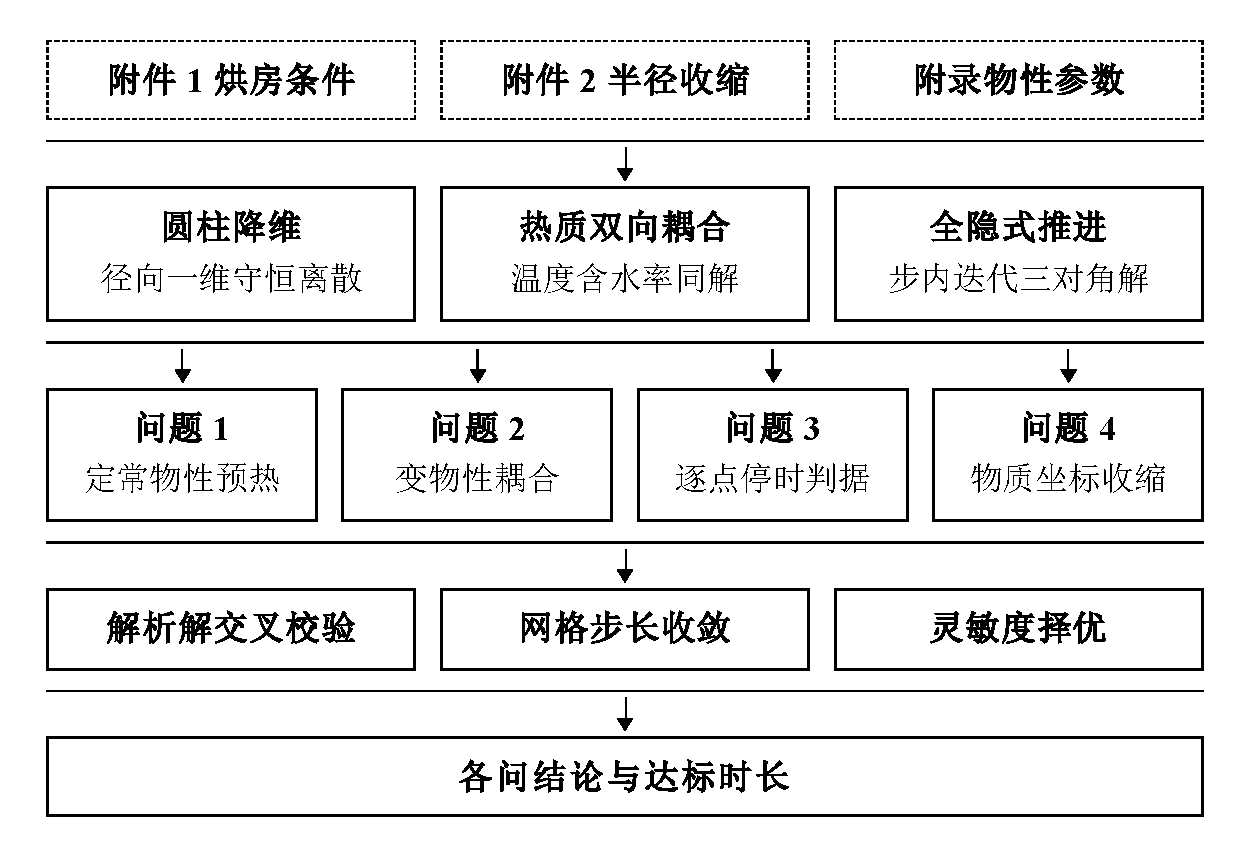
\includegraphics[width=0.8\textwidth,height=0.8\textheight,keepaspectratio]{../figures/fig_roadmap.pdf}
  \caption{全文技术路线。自上而下依次为题给数据、四问共用的数学内核、四个问题
  的分支求解、可信性校验与结论交付五层；虚线框表示题给数据，加粗框为四问共用的
  耦合内核，层间横线表示先汇总再分发；四个问题框内第二行即该问在内核之上新增的
  处理，可见四问同源而分支互不重复。}
  \label{fig:roadmap}
\end{figure}

图中第二层的耦合内核只建立一次，四条分支各自只在其上添加一项处理：问题一固定物性、固定区域，问题二把物性交给解本身决定，问题三在解之上叠加一个首次达标的判定，问题四让区域的外边界随实测半径移动。这种分层使得四问的差异可以被逐项分离，时长变化中的物性效应与几何效应因而各有对应的分支，不必混在一起解释。下面按题目编号说明各问的任务性质与建模取向。

\subsection{问题一的分析}

问题一是一个给定时变边界激励的初边值问题。药材初始温度与含水率均匀，烘房空气的温度与含湿由实测序列给定，需要求出半小时内温度场与水分场沿半径的演化。任务本身并不复杂，难点在于两个场的时间尺度相差悬殊：由该阶段的常物性算得热扩散率约为 $1.69\times10^{-7}$~m$^2$/s，而初始含水率下的水分扩散系数只有约 $4.9\times10^{-9}$~m$^2$/s，相差三十余倍。这意味着半小时之内热量已经能够穿透整个截面，水分却只在表层附近发生可观的变化，两个场必须在同一套时间推进中分别按各自的尺度求解，不能用同一个准稳态近似草率处理。

选择哪一类边界条件是本问的第一个实质判断。以对流换热系数与半径、导热系数构成的传热毕奥数约为 $1.4$，量级为一，既不允许把药材当成温度均匀的集中体，也不允许把表面温度直接取为空气温度，只有第三类边界条件才能同时容纳内部梯度与表面阻力。传质一侧的毕奥数在初始时刻约为 $3$，随着表层变干而迅速增大到千的量级，表明水分迁移由内部扩散控制，这与文献对切片类物料含水率剖面与传质毕奥数关系的分析一致\upcite{rovedo1998biot}。两者合起来决定了模型形式：圆柱坐标下的一维径向守恒方程，表面两个第三类边界，轴线零通量。求解上采用顶点式有限体积离散配合全隐式时间推进，使离散节点正好落在题目要求输出的径向位置上，同时让轴线的零通量在离散层面自动精确满足。本问确立的方程形式、边界处理与离散框架为后三问共用。

\subsection{问题二的分析}

问题二把时间跨度从半小时拉长到两三天，方程形式沿用问题一，但物性改由本阶段的经验公式给出，密度随含水率线性变化，比热容与导热系数随湿基含水率变化，扩散系数则同时含有含水率因子与温度的 Arrhenius 因子。物性一旦依赖待求解，方程就由线性变为非线性，每个时间层都需要用当前解重新计算系数并迭代到自洽，本文为此在每一步内嵌一层不动点迭代。

真正需要小心的是扩散系数的取值位置。经验式中含水率以倒数形式进入指数，表层含水率越过阈值继续下降时扩散系数会跨越四个数量级，相邻两个节点上的取值可能相差十倍以上。此时若沿用常规的算术平均或调和平均来构造控制体界面上的扩散系数，界面通量会被系统性地拉向偏大或偏小的一侧，尤其是调和平均在一侧数值极小时几乎把界面通量压至零，导致失水速率失真。本文改用沿两节点连线对扩散系数作积分平均，使离散通量与扩散势差的关系保持一致。此外经验式中的温度必须取绝对温度，若误用摄氏读数，Arrhenius 因子会被放大若干个数量级。本问输出的全过程解直接作为问题三判定停时的对象。

\subsection{问题三的分析}

问题三不引入新的物理机制，它改变的是提问方式：前两问求场的演化，本问求一个由场定义的时刻。题目要求药材各处的水分浓度都低于阈值，因而合格与否取决于全域中最湿的那一点，而不是表面读数或截面平均值。这三种可能的判据在时间轴上的触发次序是确定的：表面最先达标，截面平均次之，全域最大值最后，若误用前两者会系统性地低估所需时长。轴对称与外向失水的组合使最湿位置始终位于轴线附近，因此判据量在数值上表现为中心含水率，但其定义仍应写成径向最大值，以免在其他工况下失效。

由此本问归结为一个首次穿越时刻的确定：在离散输出的时间序列上逐点比较判据量与阈值，找到符号改变的那一个区间，再在区间内插值定位。由于判据量在阈值附近单调下降且只穿越一次，插值给出的时刻是唯一的。需要一并说明的是，停时是判据量恰好等于阈值的时刻，此刻药材最湿处的含水率等于阈值而非严格小于阈值，严格不等式在其后的任意时刻成立，交付结果的读法需要据此解释。

\subsection{问题四的分析}

问题四新增的是几何：药材因失水而收缩，半径由实测序列给出，求解区域的外边界随时间向轴线移动。前三问在固定区域上写出的方程不再直接适用，处理移动边界有两条路线，一是保留实验室坐标而让网格随边界收缩，二是引入以当前半径归一的物质坐标把区域固定下来，后者是食品与农产品干燥中处理收缩的常用途径\upcite{adrover2018moving,xanthopoulos2026mb}。本文取后者：把半径与当前半径之比作为空间自变量后，网格节点随物质一同向轴线移动，链式法则展开时坐标变换项与表观对流项恰好相消，方程中不再显式出现半径变化率，边界始终落在坐标的端点上。收缩效应则以当前半径平方的倒数进入扩散项，半径缩小意味着同样的含水率落差被压缩在更短的距离上，梯度增大，干燥因此加快。两种写法在数学上是等价的，本文用实验室坐标的写法作为独立对照来交叉检验实现的正确性。

本问时长与问题三的差异有两个来源且方向相反。物性组更换到收缩情形对应的一套后，扩散系数的前因子显著变小，单看这一项会使干燥明显变慢；几何收缩则如上所述使干燥加快。只有把两者分开计算才能说明最终时长为何仍短于问题三。另外，收缩过程中水分不断离开药材而干物质总量应保持不变，这为模型提供了一个不依赖判据的独立检验：干物质的径向积分在整个过程中是否守恒，以及由实测半径反推的干物质密度与经验公式给出的密度是否相容。
